

\documentclass[10pt]{beamer}
\usepackage{amsmath,amssymb}
\usepackage[brazil]{varioref}
\usepackage[russian,english]{babel}
\usepackage[utf8]{inputenc}
\usetheme{default}
\usepackage{mathtools}
\usepackage{multirow}
\mathtoolsset{showonlyrefs}



\definecolor{cvut_navy}{HTML}{0065BD}
\definecolor{cvut_blue}{HTML}{6AADE4}
\definecolor{cvut_gray}{HTML}{156570}

% \setbeamercolor{section in toc}{fg=black,bg=white}
% \setbeamercolor{alerted text}{fg=cvut_blue}
% \setbeamercolor*{palette primary}{bg=cvut_navy,fg=gray!20!white}
% \setbeamercolor*{palette secondary}{bg=cvut_blue,fg=white}
% \setbeamercolor*{palette tertiary}{parent=palette primary}
% \setbeamercolor*{palette quaternary}{fg=green,bg=gray!5!white}

% \setbeamercolor*{sidebar}{fg=cvut_navy,bg=gray!15!white}


% \setbeamercolor{titlelike}{parent=palette primary}
% \setbeamercolor{frametitle}{parent=palette primary}

% \setbeamercolor*{separation line}{}
% \setbeamercolor*{fine separation line}{}

\setbeamertemplate{navigation symbols}{} 


\usepackage{amsmath, amssymb, amsfonts}
\usepackage[utf8]{inputenc}
\usepackage{movie15}
\usepackage[T2A]{fontenc}
\usepackage{graphicx}
\usepackage{subfig}
\usepackage[noend]{algorithmic}
\usepackage{tikz}
\usepackage{amsmath,amsfonts,amsthm,amssymb,amsbsy,amstext,amscd,amsxtra,multicol}
\usepackage{verbatim}
\usetikzlibrary{automata,positioning}
\usepackage{multicol}
\usepackage{graphicx}


\usepackage{appendixnumberbeamer}
%\usecolortheme{dove}
%\usefonttheme{serif}

\newcommand{\cond}{\mspace{3mu}{|}\mspace{3mu}}
\newcommand{\norm}{\mathop{\rm norm}\limits}
\newcommand{\tsum}{\mathop{\textstyle\sum}\limits}
\newcommand{\tprod}{\mathop{\textstyle\prod}\limits}

\let\l\limits


\title
[Слайд \hfill\insertframenumber\,/\,\inserttotalframenumber ]
{\large Convolution, Correlation \\and\\ 
Fourier Transforms}
\author[Student Filipp Nikitin]{%
  Student Filipp Nikitin
  }
  \institute[MIPT]{
      Moscow institute of Physics and Technology
\\(state university)\\
     Phystech school of applied mathematics and informatics
     }
\date{\today}

\begin{document}

\begin{frame}
    \titlepage
    \begin{center}
          
\includegraphics[height=1.4cm]{logo_img/mipt.png} \ \ \
        
\includegraphics[height=1.4cm]{logo_img/vc-ran_logo.png}
    \end{center}
\end{frame}

\begin{frame}[t]{Plan}

\begin{enumerate}
    \item Introduction
    
    \item Fourier Transforms

    \item Convolution transform. Convolution theorem 
    
    \item Proof of the convolution theorem 
    
    \item Correlation and auto-correlation
    
    \item CNN: Advanced insights
    
    \item Bonus
    
    
    
\end{enumerate}
    
\end{frame}


\begin{frame}[t]{Time and Frequency Domains}

Two ways of process descibing:

\begin{itemize}
    \item \textbf{Time domain}. Values of some quantity
    
    \item \textbf{Frequency Domain}. Complex number: amplitude and phase 
\end{itemize}

\begin{block}{Fourier transforms}
The mapping between the domains
\end{block}

    \begin{figure}
        \centering
        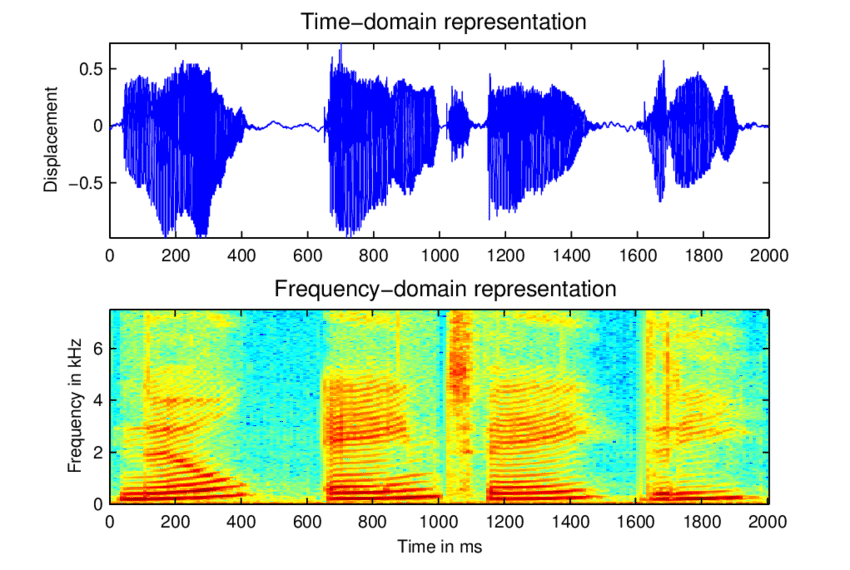
\includegraphics[width=.7\textwidth]{domains.png}
        \caption{Two representations of speech.}
    \end{figure}

\end{frame}


\begin{frame}{Fourier Transforms}

\begin{enumerate}
    \item From time domain to frequency domain:
    \begin{equation}
        H(f) = \int \limits_{-\infty}^{+\infty} h(t) \exp({-2\pi ift}) dt 
    \end{equation}
    
    \item From frequency domain to time domain:
    \begin{equation}
        h(t) = \int \limits_{-\infty}^{+\infty} H(f) \exp({2\pi ift}) df
    \end{equation}
\end{enumerate}


\begin{block}{Properties}
\begin{enumerate}
    \item FT is a linear operator
    \item Time scaling: $h(at) \equiv \frac{1}{a}H(\frac{f}{a})$
    \item Time shifting: $h(t-t_0) \equiv H(f) \exp(-2\pi ift_0)$ 
\end{enumerate}

\end{block}

    
\end{frame}


\begin{frame}{Convolution}
Functions $h(t)$ and $g(t)$ is given. $H(f)$ and $G(f)$ are corresponding Fourier transforms. 

\medskip

\begin{block}{Convolution}
\begin{equation}
    f(t) = g * h \equiv \int \limits_{-\infty}^{+\infty} f(v) g(t - v) dv 
\end{equation}

For functions f, g supported on only $[0, \infty)$, the integration limits can be truncated:

\begin{equation}
    f(t) = g * h \equiv \int \limits_{0}^{t} f(t- v) g(v) dv 
\end{equation}

\end{block}

\begin{block}{Properties:}

\begin{itemize}
    \item $g*h = h*g$
    \item $g*h \equiv G(f)H(f)$
\end{itemize}

\end{block}

\end{frame}

\begin{frame}{Convolution Theorem}

\begin{block}{Theorem}

The Fourier transform of the convolution is the product of the two Fourier transforms.

\begin{align}
    \mathcal{F}(f*g) = \mathcal{F}(f)\mathcal{F}(g)
\end{align}

Where $\mathcal{F}$ is a Fourier transform.

\end{block}

\begin{block}{Modifications:}
\begin{enumerate}
    \item Laplace transform \\
    \item Two-sided Laplace transform\\
    \item Z-transform \\
    \item Mellin transform
\end{enumerate}
\end{block}
    
\end{frame}

\begin{frame}{Proof for Laplace transform}

\begin{block}{Laplace transform:}
\begin{equation}
    \mathcal{L}(f) = \int \limits_0^\infty \exp(-st) f(t)dt  
\end{equation}
\end{block}

\begin{block}{Convolution theorem:}
\begin{equation}
    \mathcal{L}(f*g) = \mathcal{L}(f)\mathcal{L}(g)
\end{equation}
\end{block}

\begin{block}{Proof:}
\begin{align}
    \mathcal{L}(f*g) &= \int \limits_0^\infty \exp(-st) \left(\int \limits_0^t f(t - v) g(v) dv \right) dt  =\\
    &= \int \limits_0^\infty \exp(-st) \left(\int \limits_0^\infty f(t - v) g(v) u(t -v) dv \right) dt
\end{align}

Where $u(t)$ is unit step function: $u(t) = \mathbb{I}(t > 0)$
\end{block}
    
\end{frame}


\begin{frame}{Proof}



\begin{align}
    \mathcal{L}(f*g) &= \int \limits_0^\infty \exp(-st) \left(\int \limits_0^\infty f(t - v) g(v) u(t -v) dv \right) dt =\\
    &= \int \limits_0^\infty \left(\int \limits_0^\infty \exp(-st)  f(t - v) g(v) u(t -v) dv \right) dt =\\
    &= \int \limits_0^\infty \left(\int \limits_0^\infty \exp(-st)  f(t - v) g(v) u(t -v) dt \right) dv =\\
    &= \int \limits_0^\infty g(v) \left(\int \limits_0^\infty \exp(-st)  f(t - v) u(t -v) dt \right) dv
\end{align}





    
\end{frame}


\begin{frame}{Proof}

Note:

\begin{equation}
    \mathcal{L}(f(t-v)u(t-v)) = \exp(-vs) \mathcal{L} (f(t)) = \exp(-vs) F(s)
\end{equation}

Then:

\begin{align}
    \mathcal{L}(f*g) &= \int \limits_0^\infty g(v) \exp(-sv) F(s) dv = F(s) G(s) = \mathcal{L}(f(t))\mathcal{L}(g(t))
\end{align}

    
\end{frame}


\begin{frame}{Correlation}

\begin{block}{Definition}
    The correlation of $g$ and $h$.  $H(f)$ and $G(f)$ are corresponding Fourier transforms. 
    
    \begin{equation}
        Corr(g, h) \equiv \int \limits_{-\infty}^{+\infty} g(v+t)h(t) dv
    \end{equation}
\end{block}

\begin{block}{Correlation theorem:}
\begin{equation}
    Corr(g, h) \equiv G(f) H^{*}(f)
\end{equation}

If $g$ and $h$ are real: $H(-f) = H^{*}(f)$.    
\end{block}

\begin{block}{Wiener-Khinchin Theorem:}
The correlation of a function with itself is
called its autocorrelation. 

\begin{equation}
    Corr(g, g) \equiv |G(f)|^2
\end{equation}
\end{block}
\end{frame}


\begin{frame}{Example of Image transform}

\begin{figure}
    \centering
    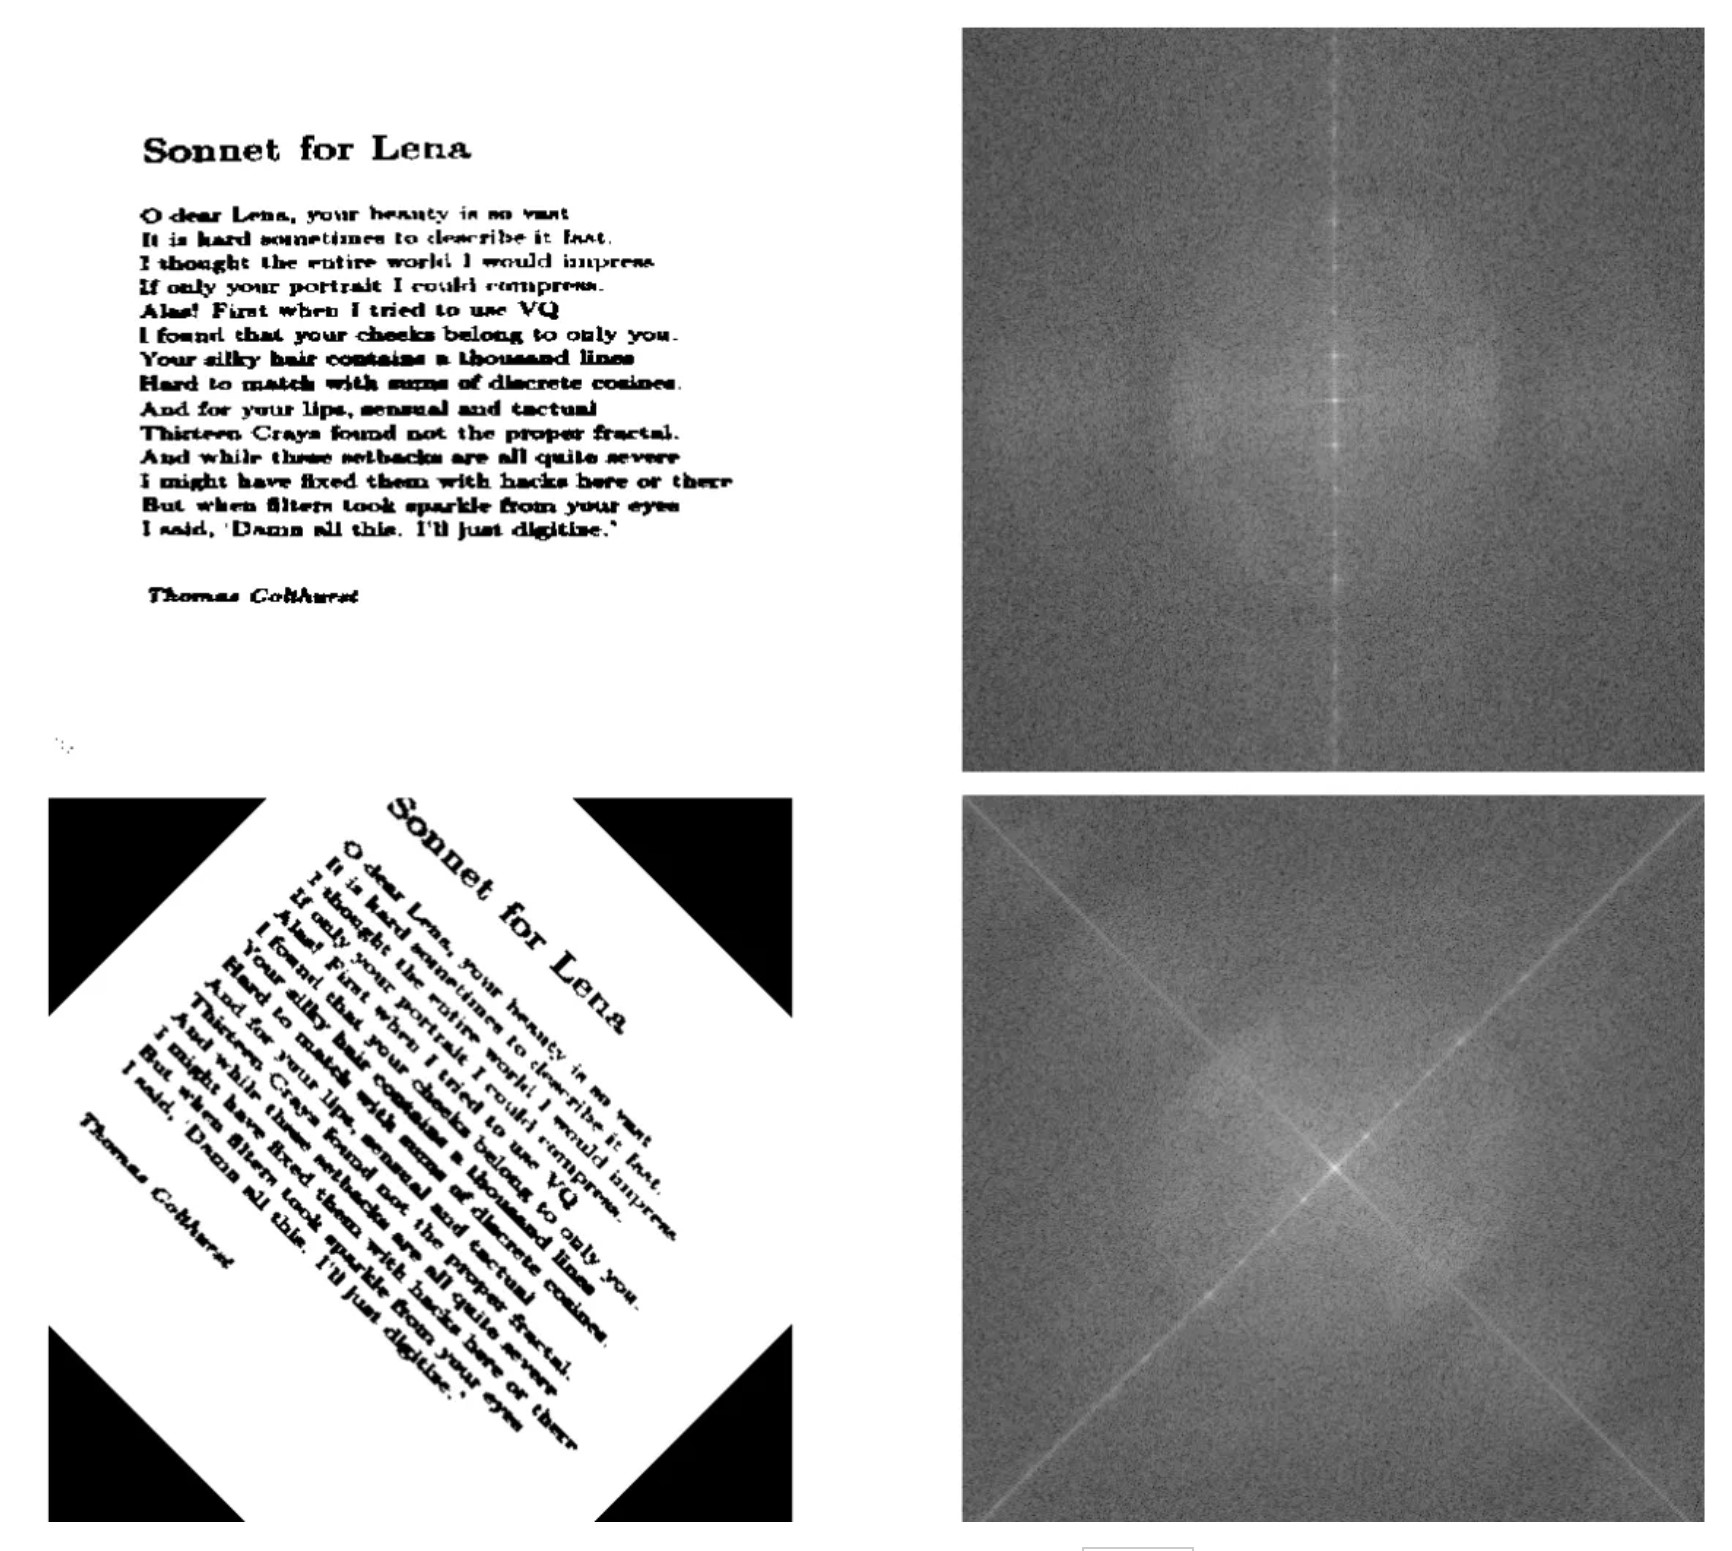
\includegraphics[width=0.7\textwidth]{fourier.jpg}
\end{figure}
    
\end{frame}



\begin{frame}{CNN: Advanced concepts}

\begin{block}{Continuous form:}

\begin{equation}
    h(x) = f * g = \int \limits_{-\infty}^{\infty} f(x - v) g(v) dv = \mathcal{F}^{-1}(\mathcal{F}(f) \mathcal{F}(g))
\end{equation}

\end{block}

\begin{block}{Discrete form:}

\begin{align}
    y[m, n] &= h[m, n] *\; x[m, n] = \sum \limits_{-\infty}^{\infty} \sum \limits_{-\infty}^{\infty} h[i, j]\; x[m-i, n-j] = \\
      &= \mathcal{F}^{-1}(\mathcal{F}(x) \mathcal{F}(k))
\end{align}

\end{block}

\begin{block}{Note}

A Fourier transform contains a lot of information about the orientation of an object in an image.

\end{block}

\textbf{Open question}:

Can we imagine that convolutional nets operate on images in the Fourier domain?

\end{frame}


\begin{frame}{CNN: Cross-correlation}
    Cross-correlation for real functions $g, h$: 
    \begin{equation}
        Corr(g, h) \equiv G(f) H(-f)
    \end{equation}
    
    \begin{figure}
        \centering
        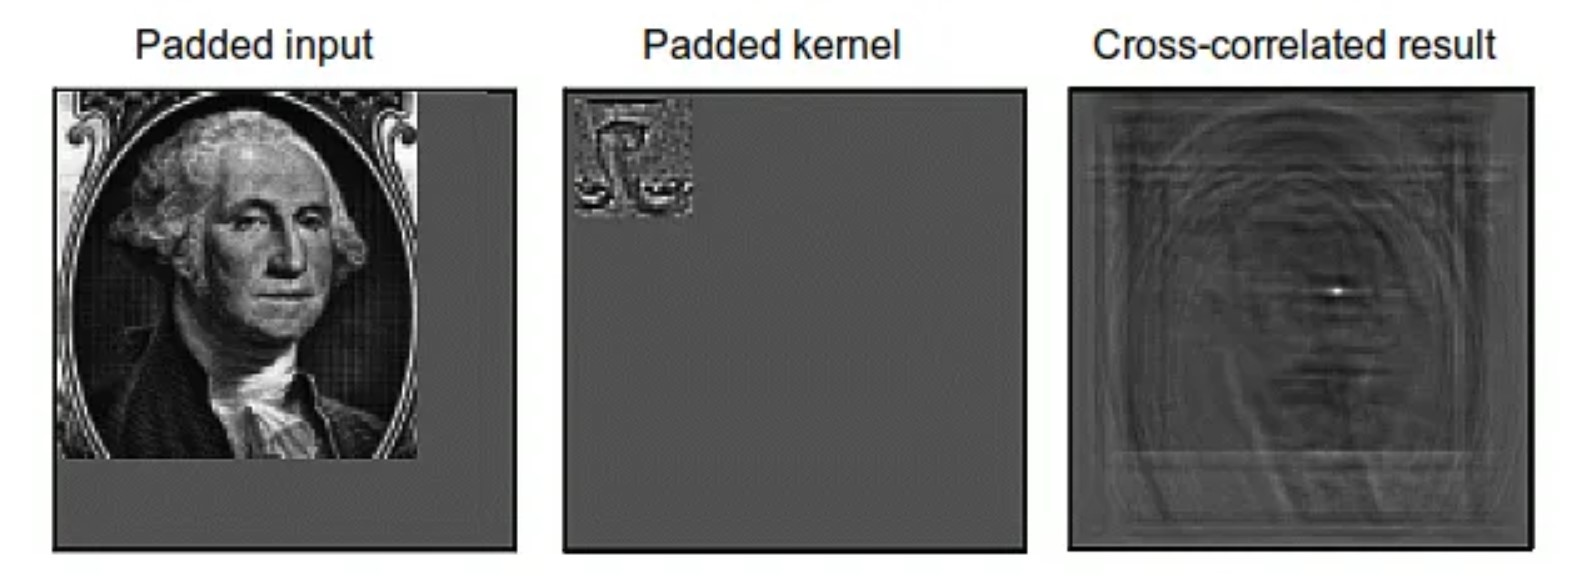
\includegraphics[width=0.8\textwidth]{corr.jpg}
        \caption{Cross-correlation via convolution: The input and kernel are padded with zeros and the kernel is rotated by 180 degrees. }
    \end{figure}
\end{frame}


\begin{frame}{Bonus: Complex networks}

\textbf{Reasons}:

\begin{enumerate}
    \item Improve phase prediction in existed pipelines 
    \item Work directly in Fourier domain
    \item Use previously developed theory
\end{enumerate}

\begin{figure}
    \centering
    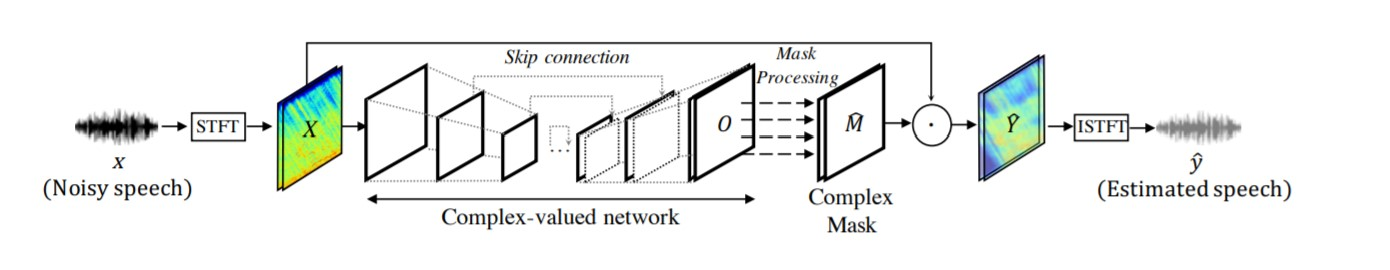
\includegraphics[width=\textwidth]{complex.jpg}
    \caption{Deep complex U-net}
    \label{fig:my_label}
\end{figure}

\end{frame}

\begin{frame}{Summary}
\begin{itemize}
    \item Fourier Transform
    \item Convolution in a general view
    \item Convolution theorem with proof
    \item Convolution and cross-correlation
    \item CNN: Advanced insights
    \item Complex Networks
\end{itemize}
\end{frame}




\begin{frame}
\centering
\Large{Thank you!}
\end{frame}



{\small
\begin{frame}[allowframebreaks]{Основная литература}
    \bibliographystyle{plainnat}
    \nocite{*}
    \bibliography{demo}    
\end{frame}
}



\end{document}
